\documentclass[10pt]{article}

\usepackage[margin=0.75in]{geometry}
\usepackage{amsmath,amsthm,amssymb,bm}
\usepackage{xcolor}
\usepackage{cancel}
\usepackage{graphicx}
\usepackage{changepage}
\usepackage{circuitikz}
\usepackage{pgfplots}
\usepackage{minted}
\usepackage{physics}
\usepackage{tikz}
\usepackage{tikz-3dplot}
\usepackage{hyperref}
\usepackage{cleveref}
\usepackage{siunitx}
\usepackage{fontspec}
\usepackage{relsize}
\usepackage{subfig}
\usepackage{todonotes}
\usepackage{contour}
\usepackage{multicol, multirow, booktabs}
\usepackage[breakable]{tcolorbox}
\usepackage[inline]{enumitem}

\theoremstyle{definition}
\newtheorem{problem}{Problem}
\newtheorem{soln}{Solution}

\pgfplotsset{compat=newest}
\usetikzlibrary{lindenmayersystems}
\usetikzlibrary{arrows}
\usetikzlibrary{calc}
\usetikzlibrary{positioning, fit}
\usetikzlibrary{3d, perspective}
\usetikzlibrary{math}
\usetikzlibrary{fadings}
\usetikzlibrary{angles,quotes} 
\usetikzlibrary{decorations.markings}

\definecolor{incolor}{HTML}{303F9F}
\definecolor{outcolor}{HTML}{D84315}
\definecolor{cellborder}{HTML}{CFCFCF}
\definecolor{cellbackground}{HTML}{F7F7F7}
\newcommand{\ui}{\hat{i}}
\newcommand{\uj}{\hat{j}}
\newcommand{\uk}{\hat{k}}
\newcommand{\ux}{\hat{\mathbf{x}}}
\newcommand{\uy}{\hat{\mathbf{y}}}
\newcommand{\uz}{\hat{\mathbf{z}}}
\newcommand{\uv}[1]{\hat{\bv{{#1}}}}
\newcommand{\pr}[1]{{#1^\prime}}
\newcommand{\pd}[2][]{{\frac{\partial^{#1}}{\partial {{#2}^{#1}}}}}
\newcommand{\dif}[2][]{{\frac{d^{#1}}{d{{#2}^{#1}}}}}
\newcommand{\grd}{\nabla}

\pgfdeclarelayer{background}  
\pgfsetlayers{background,main}
\AtBeginDocument{\RenewCommandCopy\qty\SI}

\makeatletter
\newcommand{\boxspacing}{\kern\kvtcb@left@rule\kern\kvtcb@boxsep}
\makeatother
\newcommand{\prompt}[4]{
    \ttfamily\llap{{\color{#2}[#3]:\hspace{3pt}#4}}\vspace{-\baselineskip}
}

\newcommand{\thevenin}[2]{
  \begin{center}
    \begin{circuitikz} \draw
      (0,0) -- (2,0) to[battery1, l_=$V_{Th}\eq#1$] (2,2) 
      to[resistor, l_=$R_{Th}\eq#2$] (0,2)
      ;
      \draw [o-] (-.07,2.079);
      \draw [o-] (-.07,0.079);
    \end{circuitikz}
  \end{center}
}

\newcommand{\norton}[2]{
  \begin{center}
    \begin{circuitikz} \draw
      (0,0) -- (3,0) to[american current source, l_=$I_{N}\eq#1$] (3,2) -- (0,2) (2,0)
      to[resistor, l=$R_{N}\eq#2$] (2,2)
      ;
      \draw [o-] (-.07,2.079);
      \draw [o-] (-.07,0.079);
    \end{circuitikz}
  \end{center}
}

\DeclareMathOperator{\Div}{div}
\DeclareMathOperator{\Curl}{curl}
\DeclareMathOperator{\sgn}{sgn}

\newcommand{\highlight}[1]{\colorbox{yellow}{$\displaystyle #1$}}
\newcommand{\ti}[1]{\widetilde{#1}}
\renewcommand{\div}[1]{\bv{\nabla}\cdot #1}
\renewcommand{\curl}[1]{\bv{\nabla}\times #1}

\newfontface{\Kaufmann}{Kaufmann}
\DeclareTextFontCommand{\kf}{\Kaufmann}
\newcommand{\scriptr}{\fontsize{12pt}{12pt}\kf{r}\fontsize{10pt}{10pt}}

\newfontface{\KaufmannB}{Kaufmann Bold}
\DeclareTextFontCommand{\kfb}{\KaufmannB}
\newcommand{\bscriptr}{\fontsize{12pt}{12pt}\kfb{r}\fontsize{10pt}{10pt}}
\newcommand{\justif}[2]{&{#1}&\text{#2}}
\newcommand{\bv}[1]{\bm{\mathrm{#1}}}

\title{Physics 4240H: Assignment II}
\author{Jeremy Favro (0805980) \\ Trent University, Peterborough, ON, Canada}
\date{\today}

\begin{document}
\maketitle

% PROBLEM 1
\begin{problem}
\begin{enumerate}[label=(\alph*)]
  \item Depict using a phasor diagram the following two harmonic oscillations at point $P$:
        $$E_1(P,t)=2\cos\omega t\quad\text{and}\quad E_2(P,t)=7\cos(\frac{\pi}{3}-\omega t).$$
  \item Determine from this phasor approach the expression for the resultant disturbance.
  \item Confirm that the same result stems from a purely algebraic approach.
\end{enumerate}
\end{problem}
\begin{soln}
  \begin{enumerate}[label=(\alph*)]
    \item We begin by writing the fields in complex form,
          $$E_1(P,t)=\Re{2e^{-i\omega t}}\quad\text{and}\quad E_2(P,t)=\Re{7e^{i(\frac{\pi}{3}-\omega t)}}=\Re{7e^{i\pi/3}e^{-\omega t}}$$
          (note that change to $-\omega t$ in the first term, this makes factoring easier and doesn't affect the cosine as cosine is even)
          and hence their sum is
          $$E_R(P,t)=\Re{\left(2+7e^{i\pi/3}\right)e^{-i\omega t}}.$$
          Plotting the non-oscillating (in time) part on the Argand plane,
          \begin{center}
            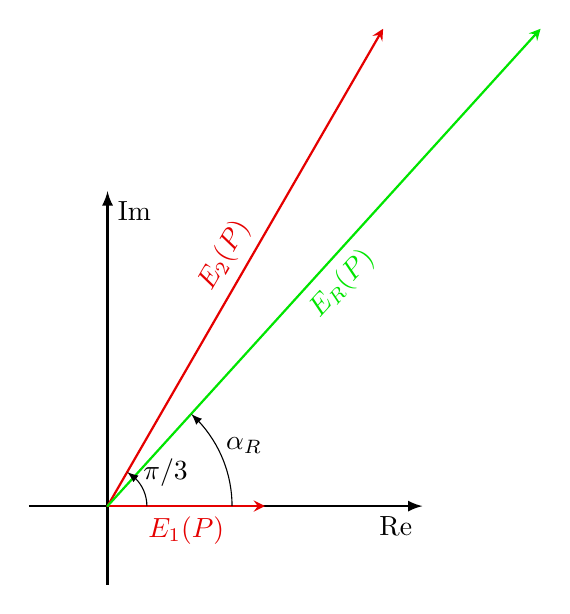
\begin{tikzpicture}
              \tikzset{>=latex}
              \tikzstyle{vector}=[-stealth,red!90!black,thick,line cap=round]
              \tikzstyle{rvector}=[-stealth,green!90!black,thick,line cap=round]

              % CONSTANTS
              \coordinate (O) at (0,0);
              \draw[thick,->] (-1,0) -- (4,0) node[anchor=north east]{Re};
              \draw[thick,->] (0,-1) -- (0,4) node[anchor=north west]{Im};

              \draw[vector] (O) -- ({2},{0}) node[midway, below]{$E_1(P)$} coordinate (A);
              \draw[vector] (O) -- ({7*cos(deg(pi/3))},{7*sin(deg(pi/3))})
              node[midway, above, rotate={180/3}]{$E_2(P)$} coordinate (B);
              \draw[rvector] (O) -- ({2+7*cos(deg(pi/3))},{7*sin(deg(pi/3))}) node[midway, below, rotate={atan((7*sin(deg(pi/3)))/(2+7*cos(deg(pi/3))))}]{$E_R(P)$} coordinate (C);
              \pic [draw, ->, "$\pi/3$", angle eccentricity=1.7] {angle = A--O--B};
              \pic [draw, ->, "$\alpha_R$", angle eccentricity=1.2, angle radius=45] {angle = A--O--C};
            \end{tikzpicture}
          \end{center}
    \item Evidently to obtain the components of the resultant phasor we just take add the real and imaginary components of the inputs as if they were vector components.
          The real components are $2$ and $7\cos(\pi/3)=7/2$ and the imaginary components are $0$ and $7\sin(\pi/3)=7\sqrt{3}/2$ and hence the
          resultant phasor is
          $$\left[(2+\frac{7}{2})+\frac{7\sqrt{3}}{2}i\right]=\frac{1}{2}\left[11+7\sqrt{3}i\right]$$
          with angle
          $$\alpha_R=\arctan(7\sqrt{3}/11)\approx 0.83$$
          and magnitude $\sqrt{67}$
          which gives a resultant wave of
          $$E_R(P,t)\approx \Re{\sqrt{67}e^{0.83i}e^{-i\omega t}}=\sqrt{67}\cos(0.83-\omega t).$$
    \item Purely algebraic?
  \end{enumerate}
\end{soln}

% PROBLEM 2
\begin{problem}
Plot and write the equation for the superposition of the following harmonic oscillations at point $P$:
$$E_1(P,t)=\sin(\frac{\pi}{18}-\omega t),\quad E_2(P,t)=3\cos(\frac{5\pi}{9}-\omega t),\quad E_3(P,t)=2\sin(\frac{\pi}{6}-\omega t)$$
where the period of each oscillation is $\qty{2}{\second}$.
\end{problem}
\begin{soln} To sum these waves algebraically we require that they all be cosines for convenience. This means we subtract $\pi/2$ from
  each of the $\sin$ arguments. We then rewrite the waves in complex form,
  $$E_R(P,t)=\Re{\left[\cos(4\pi/9)-i\sin(4\pi/9)+3\cos(5\pi/9)+3i\sin(5\pi/9)+2\cos(\pi/3)-2i\sin(\pi/3)\right]e^{-i\omega t}}$$
  This makes it (somewhat) clear that the amplitude of the resultant will be
  $$E_{0R}=\sqrt{(\cos(4\pi/9)+3\cos(5\pi/9)+2\cos(\pi/3))^2+(-\sin(4\pi/9)+3\sin(5\pi/9)-2\sin(\pi/3))^2}\approx 0.69$$
  and that the angle will be
  $$\alpha_R=\arctan(\frac{-\sin(4\pi/9)+3\sin(5\pi/9)-2\sin(\pi/3)}{\cos(4\pi/9)+3\cos(5\pi/9)+2\cos(\pi/3)})\approx 0.35$$
  and so the resultant wave is
  $$E_R(P,t)\approx 0.69\cos(0.35-\omega t).$$
  \begin{figure}[h]
    \centering
    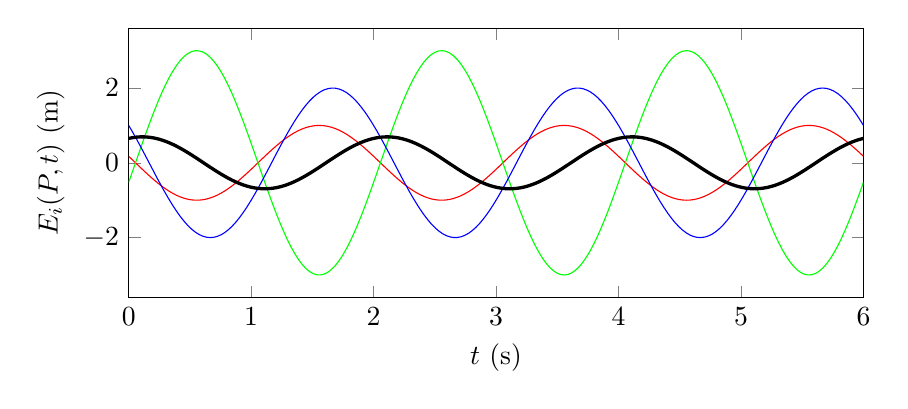
\begin{tikzpicture}
      \begin{axis}[
          width=\textwidth*0.9, height = 5cm,
          xlabel={$t$ (s)}, ylabel={$E_i(P,t)$ (m)},
          xmin=0, xmax=6
        ]
        \addplot[domain=0:6, samples=200, color=red](\x,{sin(deg(pi*((1/18)-\x)))});
        \addplot[domain=0:6, samples=200, color=green](\x,{3*cos(deg(pi*((5/9)-\x)))});
        \addplot[domain=0:6, samples=200, color=blue](\x,{2*sin(deg(pi*((1/6)-\x)))});
        \addplot[domain=0:6, samples=200, color=black, very thick](\x,{sin(deg(pi*((1/18)-\x)))+3*cos(deg(pi*((5/9)-\x)))+2*sin(deg(pi*((1/6)-\x)))});
      \end{axis}
    \end{tikzpicture}
    \caption{Red: $\sin(\frac{\pi}{18}-\omega t)$, green: $3\cos(\frac{5\pi}{9}-\omega t)$, blue: $2\sin(\frac{\pi}{6}-\omega t)$. Black is the result
      from summing red, green, and blue.}
  \end{figure}
\end{soln}

% PROBLEM 3
\begin{problem}
Standing waves are produced by the superposition of the wave given below and its perfect reflection from a mirror. Here, the disturbance is an electric field given in units of
$\unit{\kilo\volt\per\meter}$, while time $t$ is in seconds and distance $x$ is in $\unit{\centi\meter}$:
$$E(x,t)=7\sin\left[2\pi\left(\frac{t}{T}-\frac{2x}{\pi}\right)\right].$$
For the resultant wave, find the amplitude, wavelength, distance between nodes, velocity, and period.
\end{problem}
\begin{soln}
  The reflected wave will be
  $$E'(x,t)=7\sin\left[-2\pi\left(\frac{t}{T}+\frac{2x}{\pi}\right)+\pi\right].$$
  The resultant wave is then
  $$E_R(x,t)=7\left[\sin\left[2\pi\left(\frac{t}{T}-\frac{2x}{\pi}\right)\right]+\sin\left[-2\pi\left(\frac{t}{T}+\frac{2x}{\pi}\right)+\pi\right]\right]$$
  which, using the identity
  $$\sin(A)+\sin(B)=2\sin(\frac{A+B}{2})\cos(\frac{A-B}{2})$$
  from the formula sheet, becomes
  $$E_R(x,t)=14
    \sin(\frac{2\pi\left(\frac{t}{T}-\frac{2x}{\pi}\right)-2\pi\left(\frac{t}{T}+\frac{2x}{\pi}\right)+\pi}{2})
    \cos(\frac{2\pi\left(\frac{t}{T}-\frac{2x}{\pi}\right)+2\pi\left(\frac{t}{T}+\frac{2x}{\pi}\right)-\pi}{2})$$
  which simplifies down to
  $$E_R(x,t)=14
    \sin(\frac{\pi-4x}{2})
    \cos(\frac{4\pi\frac{t}{T}-\pi}{2})=14\cos(4x)\sin(\frac{2\pi}{T}t).$$
  Evidently the new wave has amplitude $\qty{14}{\kilo\volt\per\meter}$, wavelength $\pi/2\,\unit{\centi\meter}$, period $T$, and velocity $\pi/2T\,\unit{\centi\meter\per\second}$.
  Nodes occur wherever $\cos(4x)=0$ and so a spacing of $3\pi/8$ (there are $3\pi/8\,\unit{\centi\meter}$ between nodes).
\end{soln}

% PROBLEM 4
\begin{problem}
The \emph{dispersive power} of glass is defined as the ratio $(n_F-n_C)/(n_D-1)$, where $C$, $D$, and $F$ refer to the
Fraunhofer wavelengths $\lambda_{0,C}=\qty{6563}{\angstrom}$, $\lambda_{0,D}=\qty{5890}{\angstrom}$, and $\lambda_{0,F}=\qty{4861}{\angstrom}$.
Find the approximate group velocity of a light pulse centered at the Fraunhofer $D$ line within glass whose dispersive power is $1/30$
and for which $n_D=1.5$.
\end{problem}
\begin{soln}
  Assuming Fraunhofer wavelengths are ordered sensibly (alphabetically), then we can apply
  $$v_g=\eval{\frac{c}{n-\lambda\frac{dn}{d\lambda}}}_{\lambda_{\text{pk}}}.$$
  Using the given information we can approximate the derivative by solving for $\Delta n=n_F-n_C$
  $$(n_F-n_C)/(1.5-1)=\frac{1}{30}\implies \Delta n = 1/60$$
  and we can find $\Delta\lambda$ to be $\qty{-167.5}{\nano\meter}$ by subtracting the F and C wavelengths. Plugging these into the expression
  $$v_g=\frac{c}{1.5-\qty{589}{\nano\meter}\frac{1/60}{\qty{-167.5}{\nano\meter}}}\approx 0.64 c.$$
\end{soln}

% PROBLEM 5
\begin{problem} A source comprising $N$ antennas emits $N$ waves such that the wave from the $j$th antenna results
in an electric field at point $P$ given by
$$E_j(P,t)=E_0\cos(\epsilon_j-\omega t).$$
Here $E_0$ is the same for all antennas, and the phase difference between waves from adjacent antennas is a constant $\delta$ (so that $\epsilon_{j+1}-\epsilon_j=\delta$)
\begin{enumerate}[label=(\roman*)]
  \item Writing the field from each antenna in the complex form $\ti{E}_j(P,t)=E_0e^{-i\omega t}e^{i\epsilon_j}$, where $\epsilon=\epsilon_0+j\delta$,
        what is the expression for the resultant field at point $P$?
  \item What is the expression for the amplitude of this field?
  \item For $N=8$, what is the amplitude of the resultant field $P$ when the phase difference between waves is $\pi\,\unit{\radian}$?
  \item For $N=8$, what is the amplitude of the resultant field $P$ when the phase difference between waves is $0.5\,\unit{\radian}$?
\end{enumerate}
\end{problem}
\begin{soln}~\begin{enumerate}[label=(\roman*)]
    \item Summing over all waves $E_R(P,t)=\sum_{j=1}^{N}E_0e^{-i\omega t}e^{i\epsilon_j}=E_0e^{-i\omega t}e^{i\epsilon_0}\sum_{j=1}^{N}e^{ij\delta}$
          which is a geometric series and, using the identity (where I've changed indices since the usual sum starts at 0)
          $$\sum_{j=1}^{N}r^{j-1}=\frac{1-r^N}{1-r}$$
          can be rewritten as
          $$E_R(P,t)=E_0e^{-i\omega t}e^{i\epsilon_0}e^{-i\delta}\left[\frac{1-e^{iN\delta}}{1-e^{i\delta}}\right]$$
          where the $e^{-i\delta}$ accounts for the missing $r^{-1}$ term.
          Looking at the possible answers, we then factor out a half (argument) exponential from top and bottom,
          $$E_R(P,t)=E_0e^{-i\omega t}e^{i\epsilon_0}e^{-i\delta}e^{i(N-1)\delta/2}\left[\frac{e^{-iN\delta/2}-e^{iN\delta/2}}{e^{-i\delta/2}-e^{i\delta/2}}\right]$$
          and recall that $2\Im(x)=x-\overline{x}$, which is what we see in both the denominator and numerator (albeit negative and without the $2i$, but both cancel)
          so we end up with
          $$E_R(P,t)=E_0e^{-\omega t}e^{i\epsilon_0}
            e^{-i\delta}e^{i(N-1)\delta/2}\frac{\sin(\delta N/2)}{\sin(\delta/2)}
          $$
          and $e^{-i\delta}e^{i(N-1)\delta/2}=e^{i(N+1)\delta/2}$ which gives answer (D).
    \item Just by looking at the prefactor in the previous question, (A), $E_0\sin(\delta N/2)/\sin(\delta/2)$.
    \item $E_0\sin(4\pi)/\sin(\pi/2)=0$, (B).
    \item $E_0\sin(2)/\sin(1/4)\approx 3.68E_0$, (D).
  \end{enumerate}
\end{soln}
\end{document}